\documentclass{style/CRPITStyle}
\usepackage{epsfig}   % Packages to use if you wish
\usepackage{lscape}   %
\usepackage[authoryear]{natbib}
\renewcommand{\cite}{\citep}
\pagestyle{empty}
\thispagestyle{empty}
\hyphenation{roddick}

\begin{document}

\title{Software Development Life Cycles: History and Future}
\author{David Barnett}
\affiliation{School of Engineering and Computer Science \\
Victoria University of Wellington, \\
PO Box 600, Wellington, 6140 \\
Email:~{\tt barentdavi@myvuw.ac.nz}}

\maketitle

\begin{abstract}
    % TODO
    Abstract goes here
\end{abstract}

\vspace{.1in}

\noindent {\em Keywords:} Software Process Models

\vspace{.1in}

% \section{Introduction}
% TODO
% thesis statement

\section{Importance of using process models}
% Q: describe the importance of using process models to guide software development

% why we need process modeling
Fail to plan, is a plan to fail. 
As software has increased in complexity and scale of projects increase it
became more apparent that software should be managed and planned differently it was
described as a \emph{Software crisis} \cite{nato:1969}.
``We believe that the only way ahead lies through the steady development of the best existing 
techniques'' \cite{nato:1969} Gill's comments on how to move forward from the
\emph{Software Crisis} which describes a need for more of an engineering approach to software development.
One such endeavour is process modelling.
A process model is a model of how to setup a project with a set of tasks,
such as requirements acquisition or construction, of a similar nature that together form 
the scaffolding of a plan of how to approach to build a project.

\vspace{.1in} % are we allowed to do this?

By using the appropriate process model software development can be guided
through the many stages of creating software with an over-arching idea of how it
should be done. This can range from having static requirements and working
linearly through the development cycle to changing the requirements from week to
week. With the right processing model the software will have the correct tools
to handle what was expected to happen through out the process and give a guide
through the unexpected.

% add more on why it is important and how it guides

\vspace{.1in}

% TODO: this needs some reworking
Over the years many process models have been proposed and many variations have
been used and reported one. The process models that will be discussed in this
review is: Waterfall, V-Model, Spiral Model, Phased Development Model and
Extreme programming.

% --- 5 Model Section ---
% Q: provide a systematic review of process models that have been proposed so far,
% Q: compare and contract 5 selected distinct process models for software development
% Q: identify central themes that have been considered important for evolving process models
\section{Waterfall} % sequential
% theme: sequential
% strengths: requirements up front, easy
% Goals: a model of how to make successful large software
% Strengths: easy, clear steps and deliverables
% compare: ??
% contrast: ??
% note: Need a counter source, "Enough with Life cycle?"

% should include an overview & theme of the model
The Waterfall model was proposed in 1970 by Dr. Winston Royce \cite{Waterfall:1970}.
He proposed it as a method to be a guide of steps and processes that together
help to make a larger software project succeed. 
The principle idea behind the Waterfall model is that there are seven stages to
software development cycle and they are to be executed in a sequential order:
System requirements, software requirements, analysis, design, coding, testing and operations.
Each stage ends with some artifacts that the next stage depends on, forcing them
to become static, and builds upon to deliver a product at the end of the process.

\begin{figure}[htb]
\fbox{\parbox[b]{.99\linewidth}{
\vskip 0.5cm
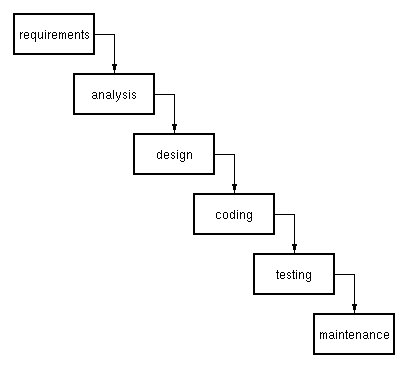
\includegraphics[width=0.45\textwidth]{figures/waterfall-model.png}
\vskip 0.5cm}}
\caption{\protect\label{xyz}  Waterfall Model}
\end{figure}

% main features of waterfall
The strength of this model lies in the assumptions that the requirements are
well thought out, any foreseeable problems has known solutions to complete the
software.
This lends the model to be more suitable for software projects that have well known
requirements and technology such as porting an application to another platform.
Waterfall also has the benefits of being an easy project to manage with its
clear milestones of development and equally easy for a new member or external
stakeholder to the team to understand the status of the project.

\vspace{.1in}

% covers the weakness of water fall
Conversely the strengths of the model also highlights the weaknesses of the model as
well.
One of the assumptions in the process model is that the requirements at the start of the project is
static and are still meet the clients needs that the project was started for.
Another factor to this weakness is that the model allows for only one delivery of the product to
the client at the end of the whole project, making a possible large time gap from requirements 
gathering with the client to the final delivery to the client which has the risk of not being 
what the client had in mind during the initial phases of the project.

\section{V-Model} % sequential, testing
% theme:
% Goals: to extends the existing Waterfall to include testing
% compare: Waterfall's steps
% contrast: Has testing involved in the 

% should include an overview & theme of the model
V-Model was proposed as a variation of the Waterfall model by Paul Rook in 1986
\cite{Rook:1986}.
The rational behind the V-Model is to produce software in a linear fashion with
well known requirements that has need for extensive testing and verification of
the system \cite{Rook:1986}.
The general workings of the V-Model are similar to the workings of Waterfall
with a few differences in testing.
Instead in V-Model the testing stage of the process model is expanded and added short loops,
the software is tested against the produced designs and requirements with
steps of verification and validations  that if failed will lead back to the design
stages or requirements respectfully.

\begin{figure}[htb]
\fbox{\parbox[b]{.99\linewidth}{
\vskip 0.5cm
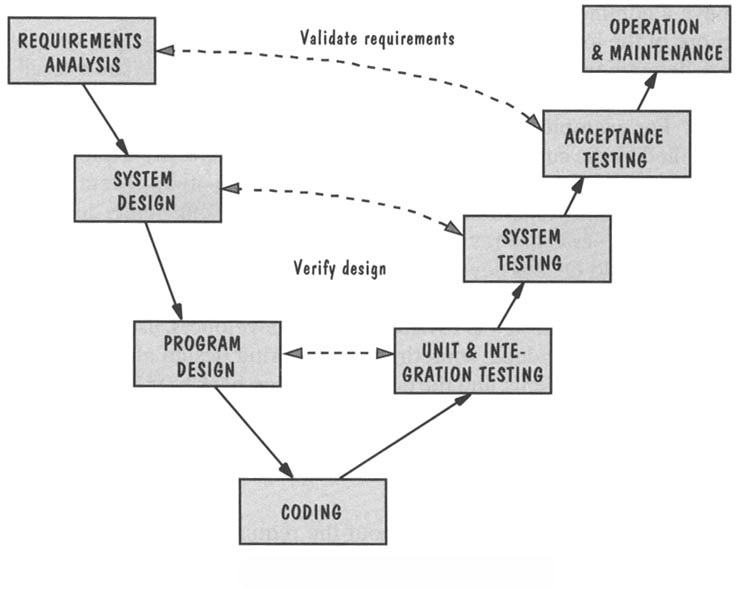
\includegraphics[width=0.45\textwidth]{figures/v-model.jpg}
\vskip 0.5cm}}
\caption{\protect\label{xyz}  V-Model}
\end{figure}

The strengths of the V-Model are built up upon Waterfall.
As with Waterfall, V-Model also is an easy to mange project with clear milestones
to each stage of development. V-Model splits off from Waterfall with its focus
on verification and validation of the product.
Through the testing the V-Model has the potential to produce an extensively well
tested product that meets a set of strict requirements such as traffic networks
or medical equipment \cite{Advancements:2010}.

The V-Model is similar to Waterfall in many aspects, such as the mainly sequential
process and having a single final derivable at the end of the process. 
The differences between the two models are highlighted with V-Model's focus towards
producing a well tested product with multiple types and opportunities to
validate and verify the program against the requirements and designs. However
both still face 


\section{Spiral Model} % sequential / Iterative, testing, risk
% theme:
% compare:
% contrast:
\cite{Boehm:1988}

\section{Phased Development Model} % iterative, testing, risk
% theme:
% compare:
% contrast:

\section{Extreme Programming} % iterative, testing, risk
% theme:
% compare:
% contrast:

\section{Possible evolutions of process models}
% Q: try to forecast how current process models may evolve in the future


\bibliographystyle{agsm}
\bibliography{essay}

\end{document}

% ------- Example Area ------
% section example
% \section{Heading Level 1}
% \subsection{Heading Level 2}
% \subsubsection{Heading Level 3}

% figure example
% \begin{figure}[htb]
% \fbox{\parbox[b]{.99\linewidth}{
% \vskip 0.5cm
% \centerline{Figure Content}
% \vskip 0.5cm}}
% \caption{\protect\label{xyz}  Caption}
% \end{figure}

% ...as proved by \citet{Snodgrass87} and \citet{FPS96} and referred to in other works \cite{BenZvi82,Bentley86,AIS93} the process..., etc.

% list example
% \begin{enumerate}
% \item Not having the correct margins -- they are 0.8 inch all round.
% \item Not using A4 paper format when creating the pdf file.
% \end{enumerate}
% vim:set spell et sw=4 ts=4 tw=80:
